% $Id: template.tex 11 2007-04-03 22:25:53Z jpeltier $

%\documentclass{vgtc}                          % final (conference style)
\documentclass[review]{vgtc}                 % review
%\documentclass[widereview]{vgtc}             % wide-spaced review
%\documentclass[preprint]{vgtc}               % preprint
%\documentclass[electronic]{vgtc}             % electronic version

%% Uncomment one of the lines above depending on where your paper is
%% in the conference process. ``review'' and ``widereview'' are for review
%% submission, ``preprint'' is for pre-publication, and the final version
%% doesn't use a specific qualifier. Further, ``electronic'' includes
%% hyperreferences for more convenient online viewing.

%% Please use one of the ``review'' options in combination with the
%% assigned online id (see below) ONLY if your paper uses a double blind
%% review process. Some conferences, like IEEE Vis and InfoVis, have NOT
%% in the past.

%% Figures should be in CMYK or Grey scale format, otherwise, colour 
%% shifting may occur during the printing process.

%% These few lines make a distinction between latex and pdflatex calls and they
%% bring in essential packages for graphics and font handling.
%% Note that due to the \DeclareGraphicsExtensions{} call it is no longer necessary
%% to provide the the path and extension of a graphics file:
%% \includegraphics{diamondrule} is completely sufficient.
%%
\ifpdf%                                % if we use pdflatex
  \pdfoutput=1\relax                   % create PDFs from pdfLaTeX
  \pdfcompresslevel=9                  % PDF Compression
  \pdfoptionpdfminorversion=7          % create PDF 1.7
  \ExecuteOptions{pdftex}
  \usepackage{graphicx}                % allow us to embed graphics files
  \DeclareGraphicsExtensions{.pdf,.png,.jpg,.jpeg} % for pdflatex we expect .pdf, .png, or .jpg files
\else%                                 % else we use pure latex
  \ExecuteOptions{dvips}
  \usepackage{graphicx}                % allow us to embed graphics files
  \DeclareGraphicsExtensions{.eps}     % for pure latex we expect eps files
\fi%

%% it is recomended to use ``\autoref{sec:bla}'' instead of ``Fig.~\ref{sec:bla}''
\graphicspath{{figures/}{pictures/}{images/}{./}} % where to search for the images

\newcommand{\squishlist}{
 \begin{list}{$\bullet$}
  { \setlength{\itemsep}{0pt}
     \setlength{\parsep}{3pt}
     \setlength{\topsep}{3pt}
     \setlength{\partopsep}{0pt}
     \setlength{\leftmargin}{1.5em}
     \setlength{\labelwidth}{1em}
     \setlength{\labelsep}{0.5em} } }


\newcommand{\squishlisttwo}{
 \begin{list}{$\bullet$}
  { \setlength{\itemsep}{0pt}
    \setlength{\parsep}{0pt}
    \setlength{	opsep}{0pt}
    \setlength{\partopsep}{0pt}
    \setlength{\leftmargin}{2em}
    \setlength{\labelwidth}{1.5em}
    \setlength{\labelsep}{0.5em} } }

\newcommand{\squishend}{
  \end{list}  }

\usepackage{algpseudocode} 
\usepackage{algorithm}
\usepackage{amsmath}
\usepackage{microtype}                 % use micro-typography (slightly more compact, better to read)
\PassOptionsToPackage{warn}{textcomp}  % to address font issues with \textrightarrow
\usepackage{textcomp}                  % use better special symbols
\usepackage{mathptmx}                  % use matching math font
\usepackage{times}                     % we use Times as the main font
\renewcommand*\ttdefault{txtt}         % a nicer typewriter font
\usepackage{cite}                      % needed to automatically sort the references
%% We encourage the use of mathptmx for consistent usage of times font
%% throughout the proceedings. However, if you encounter conflicts
%% with other math-related packages, you may want to disable it.
\usepackage{color}
\newcommand{\G}{\ensuremath{G}}
\newcommand{\V}{\ensuremath{V}}
\newcommand{\vertice}{\ensuremath{v}}
\newcommand{\weight}{\ensuremath{w}}
\newcommand{\E}{\ensuremath{E}}
\newcommand{\Hist}{\ensuremath{H}}
\newcommand{\D}{\ensuremath{D}}
\newcommand{\relevance}{\ensuremath{R}}
\newcommand{\cluster}{\ensuremath{\mathcal{C}}}
\newcommand{\watershed}{\ensuremath{\psi}}


\newcommand{\lookDan}[1]{\marginpar{---}{\color{blue}{#1}}}

\DeclareMathOperator*{\median}{\ensuremath{\text{median}}}

%% If you are submitting a paper to a conference for review with a double
%% blind reviewing process, please replace the value ``0'' below with your
%% OnlineID. Otherwise, you may safely leave it at ``0''.
\onlineid{1101}

%% declare the category of your paper, only shown in review mode
\vgtccategory{Research}

%% allow for this line if you want the electronic option to work properly
\vgtcinsertpkg

%% In preprint mode you may define your own headline.
%\preprinttext{To appear in an IEEE VGTC sponsored conference.}

%% Paper title.

\title{Visualizing demographic evolution using geographically inconsistent census data}

%% This is how authors are specified in the conference style

%% Author and Affiliation (single author).
%%\author{Roy G. Biv\thanks{e-mail: roy.g.biv@aol.com}}
%%\affiliation{\scriptsize Allied Widgets Research}

%% Author and Affiliation (multiple authors with single affiliations).
%%\author{Roy G. Biv\thanks{e-mail: roy.g.biv@aol.com} %
%%\and Ed Grimley\thanks{e-mail:ed.grimley@aol.com} %
%%\and Martha Stewart\thanks{e-mail:martha.stewart@marthastewart.com}}
%%\affiliation{\scriptsize Martha Stewart Enterprises \\ Microsoft Research}

\author{Fabio Dias\thanks{e-mail: fabio.dias@utoronto.ca} %
\and Daniel Silver\thanks{e-mail: dsilver@utsc.utoronto.ca}}
\affiliation{\scriptsize University of Toronto}

%% A teaser figure can be included as follows, but is not recommended since
%% the space is now taken up by a full width abstract.
\teaser{
  \centering
 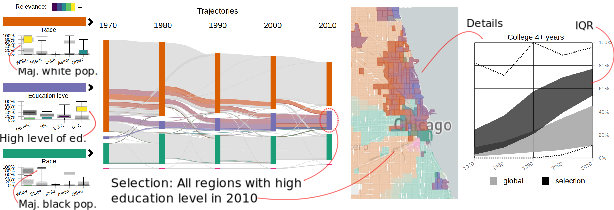
\includegraphics[width=0.85\linewidth]{newTeaser.pdf}
 \caption{Higher increase in the education level (purple cluster) in Chicago
  between 1970 and 2010. While the whole city follows this trend, the change was
  far more pronounced in these regions. The relevant clusters defined by Black
  (green) and White (orange) majority of population are also visible. 
  \label{fig:teaser}}}

%% Abstract section.
\abstract{Census measurements provide reliable demographic data going back
centuries. However, their analysis is often hampered by the lack of geographical
consistency across time. We propose a visual analytics system that enables the
exploration of geographically inconsistent data. Our method also includes
incremental developments in the representation, clustering, and visual
exploration of census data, allowing an easier  understanding of the demographic
groups present in a city and their evolution over time. We present the feedback
of experts in urban sciences and sociology, along with illustrative scenarios in
the USA and Canada.}
  
  
  % end of abstract

%% ACM Computing Classification System (CCS). 
%% See <http://www.acm.org/about/class> for details.
%% We recommend the 2012 system <http://www.acm.org/about/class/class/2012>
%% For the 2012 system use the ``\CCScatTwelve'' which command takes four arguments.
%% The 1998 system <http://www.acm.org/about/class/class/2012> is still possible
%% For the 1998 system use the ``\CCScat'' which command takes four arguments.
%% In both cases the last two arguments (1998) or last three (2012) can be empty.

\CCScatlist{ %TODO
  \CCScatTwelve{Human-centered computing}{Visu\-al\-iza\-tion}{Visualization application domains}{Visual analytics};
  \CCScatTwelve{Mathematics of computing}{Probability and statistics}{Statistical paradigms}{Exploratory data analysis
  }
}

%\CCScatlist{
  %\CCScat{H.5.2}{User Interfaces}{User Interfaces}{Graphical user interfaces (GUI)}{};
  %\CCScat{H.5.m}{Information Interfaces and Presentation}{Miscellaneous}{}{}
%}

%% Copyright space is enabled by default as required by guidelines.
%% It is disabled by the 'review' option or via the following command:
% \nocopyrightspace

%%%%%%%%%%%%%%%%%%%%%%%%%%%%%%%%%%%%%%%%%%%%%%%%%%%%%%%%%%%%%%%%
%%%%%%%%%%%%%%%%%%%%%% START OF THE PAPER %%%%%%%%%%%%%%%%%%%%%%
%%%%%%%%%%%%%%%%%%%%%%%%%%%%%%%%%%%%%%%%%%%%%%%%%%%%%%%%%%%%%%%%%
\usepackage{lineno}
\linenumbers
\begin{document}
%% The ``\maketitle'' command must be the first command after the
%% ``\begin{document}'' command. It prepares and prints the title block.

%% the only exception to this rule is the \firstsection command
\firstsection{Introduction}
\maketitle
% General context + motivation

Neighbourhoods have increasingly become a central concept in social research and
targets for social
policy~\citep{sampson2012great,galster2019making,stone2015urban,looker2015nation}.
To be sure, a focus on neighbourhoods extends to the formative period of the
modern social sciences~\citep{Abbott1997}. Recent interest has at least partly
been rekindled through newly available longitudinal demographic
datasets~\citep{Logan2014,nhgis}, convenient computational
tools~\citep{rey2018spatio}, and new sources of data~\citep{Poorthuis2018}.


\revision{In this work, we consider neighbourhoods as \emph{formal
regions}~\citep{montello2003regions}, geographically continous areas with
similar data characteristics, which these advances made more tractable to
approach in a data-driven fashion.} Yet new challenges have also emerged,
especially at the convergence of research on neighbourhood effects and
neighbourhood dynamics. Neighbourhood effects research assumes knowledge about
the nature and scope of "the neighbourhood" that presumably shapes individual
outcomes~\citep{Kwan2018,Shelton2019}. Concurrently, researchers note that
neighbourhoods are not necessarily fixed containers in which other processes
occur, but themselves dynamically
evolve~\citep{Delmelle2017,Reades2019,li2018new}. The result is to open up key
assumptions about neighbourhoods for theoretical and empirical examination: how
do we appropriately define and compare neighbourhoods at a given time?; how do
we appropriately define and compare the temporal trajectories of
neighbourhoods?; and can we do both at once, "fully
interactionally"~\citep{Abbott1997}: classify neighbourhoods now based on where
they came from and where they are going?


In principle, much of the recent research is committed to the proposition that
neighbourhoods are open and evolving entities. Ironically, its empirical
practice tends to rely on methods that require fixed geographical regions. This
requirement is difficult to satisfy, as most longitudinal datasets are based on
pre-defined tabulation areas that are routinely modified by data collection
agencies, usually to follow population changes. 

The standard approach then is to \emph{geographically harmonise} data. This
involves interpolating existing measurements into a common set of
regions~\citep{Logan2014,Hallisey2017,Allen2018}. Recent computational tools
have somewhat simplified this process~\citep{rey2018spatio}, but it still
involves non-trivial questions: which geometry to use as target, how to
apportion the variables, or how to combine data from different sources. Further,
these question do not necessarily have optimal answers. Indeed, regardless of
how well this process is performed, it still introduces
errors~\citep{Logan2016}, even when additional data is
provided~\citep{eicher2001dasymetric}. Essentially, harmonisation generates
artificial data points that can potentially lead to inaccurate results, even
though they are seldom interpreted as such. Nevertheless, because there has been
no viable alternative, and the results often appear plausible, these concerns
are generally overlooked. The result is that the harmonisation approach is
virtually mandatory in the current literature: \emph{"(...) tract-by-tract
comparison is not possible unless data from 2000 is interpolated to 2010
boundaries (...)"}~\citep{Dmowska2017}, \emph{"(...) This limits cross-year
comparison since data are not representative of the same spatial units. (...)"}
~\citep{Allen2018}. 


The main contribution of this paper is a method for longitudinal data processing
that works with the original data by leveraging a network based representation.
It enables tract-by-tract comparison and the identification of patterns of
demographic evolution \emph{without geographic harmonisation}. 

To allow a proper examination of our method and its results, we built an online
interactive system using this representation. It enables users to visualise,
interpret, and explore trajectories of neighbourhood change. This interface
helps validate our method, by allowing it to be compared to existing and future
methods. Further, it is a significant contribution to the research community: it
provides a vehicle for quickly and easily grasping complex long-term changes,
experimenting with different parameters to interactively learn from data, and
making neighbourhood change research publicly transparent. The interface thus
responds to increasing concerns about reproducibility and transparency, as well
as ongoing attention to the value of visualisation in scientific research and
communication.


We start by presenting an intuitive example of our representation in
Section~\ref{sec:introduction}, then we review the relevant literature on
longitudinal studies, data representation, clustering, and spatio-temporal
visualisation in Section~\ref{sec:related}. Our methodology is introduced in
detail in Section~\ref{sec:method}, along with the included interface.
Illustrative scenarios for Chicago, Toronto, and Los Angeles are presented in
Section~\ref{sec:study} and the feedback of five field experts are summarised in
Section~\ref{sec:expert}. Our prototype system is available at
\censure{\url{http://uoft.me/piccard}}, including more than forty regions in the
US and Canada. The source code is publicly available at
\censure{\url{https://github.com/fabioasdias/piccard}}.\footnote{The editors are
considering, at our request, an exception to the double-blind requirement to
allow access to the system. We provided them with the URLs of the system, code,
and documentation separately.}


\section{Intuition}
\label{sec:intuition}
While utterly simple, the network model breaks from the deeply rooted
traditional tabular paradigm in a significant way. The traditional method
requires the data to be treated as a collection of fixed entities with
properties that evolve over time -- rows in a table with temporal values as
columns. By contrast, our method represents each measurement as a separate
entity and encodes the evolution of these entities over time.

To ease the cognitive transition to a new paradigm, we start with an intuitive
example of how the method works, using a small portion of a fictitious urban
region illustrated on the left part of Figure~\ref{fig:intuition}. This example
includes three different times ($t_0,t_1,t_2$), with different aggregation areas
identified as letters from A to H. For $t_0$, the initial time, we have areas A
and B, with small houses and a park, respectively. The park remains stable (B,
E, and H), but the houses are partially replaced by larger buildings (C and F). 

This example illustrates some of the challenges of harmonisation. None of these
aggregation areas is clearly suitable as an interpolation target. In fact,
adopting any of these areas as a target would require merging heterogeneous
regions and/or dividing homogeneous regions. For instance, by choosing the
regions of $t_1$, A would be split to match regions C and D, which appears to be
a rather reasonable approximation in this homogeneous artificial example (even
if it commits the fallacy of division). Region F would be similarly split to
match C, but F would be split and merged with G to match D, potentially leading
to statistical measurements that do not properly represent either region. 

Real world measurements are seldom as homogeneous and noise-free as this
artificial example. By splitting and merging the data to fit arbitrary borders,
that were not necessarily coherent at the time of the measurement, harmonisation
increases the distance between measurement and reality.


\begin{figure}
    \centering 
    \subfloat{
        \includegraphics[width=0.475\linewidth]{intuition.png}
    }
    \subfloat{
        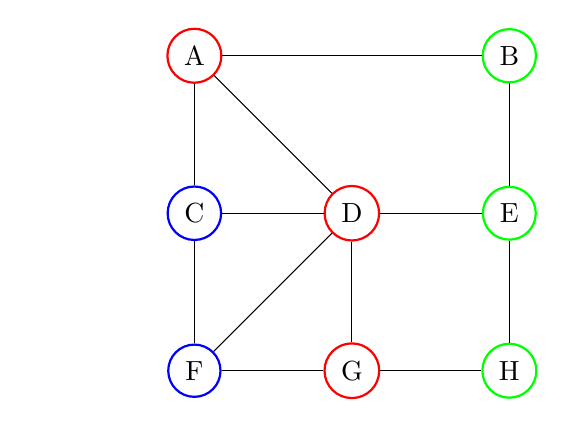
\begin{tikzpicture}
            \node (push) at (-2,0) {};
            \node [circle, draw=red, thick] (a) at (0,4) {A};
            \node [circle, draw=green, thick] (b) at (4,4) {B};
            \node [circle, draw=blue,  thick] (c) at (0,2) {C};
            \node [circle, draw=red, thick] (d) at (2,2) {D};
            \node [circle, draw=green, thick] (e) at (4,2) {E};
            \node [circle, draw=blue, thick] (f) at (0,0) {F};
            \node [circle, draw=red, thick] (g) at (2,0) {G};
            \node [circle, draw=green, thick] (h) at (4,0) {H};
            \draw (a) -- (c);
            \draw (a) -- (b);
            \draw (a) -- (d);
            \draw (b) -- (e);
            \draw (c) -- (f);
            \draw (c) -- (d);
            \draw (d) -- (f);
            \draw (d) -- (e);
            \draw (d) -- (g);
            \draw (e) -- (h);
            \draw (f) -- (g);
            \draw (g) -- (h);
        \end{tikzpicture}
    } \caption{Network based spatio-temporal data representation. \textbf{Left}:
    Three temporal stages of the evolution of a fictitious urban area, with
    aggregation areas A to H. \textbf{Right}: Network representation of the
    aggregation areas where the colours identify similar regions.
        \label{fig:intuition}}
\end{figure}

Instead, we propose a network-based representation. A \emph{network} (also
called a \emph{graph}) is a collection of entities (nodes) that are related to
each other (edges). In this case, each different aggregation area is represented
as a node and we connect nodes that have overlapping geographical areas\revision{ in
different times or are neighbours in the same time}, leading to the network
illustrated on the right of Figure~\ref{fig:intuition}. By partitioning the
network into connected nodes that are similar, we are effectively identifying
clusters in the spatio-temporal data, as illustrated by the colours of the nodes
on the right side of Figure~\ref{fig:intuition}. Further, all the possible paths
of change can be obtained by computing sequences of nodes over time, in this
case: (A, C, F), (A, D, F), (A, D, G), and (B, E, H). This representation is
also suited for geographically consistent regions, as illustrated by the stable
park in this example, and is therefore a generalisation of the traditional
paradigm.

%I'm adding this because Jeff Allen (Farber's guy) struggled with this.
Note that the edges of this network merely encode that two regions are related.
This is binary information, there is no apportionment, no areal measurements,
no population percentages associated with the edge. Indeed, our method also
connects regions of the same time that share borders, representing exactly that
they are neighbouring areas.

In the following, we argue that this network representation allows us to study
neighbourhood change in a way that does not require an prior interpolation. 

%% \section{Introduction} %for journal use above \firstsection{..} instead

\section{Related Work}

Since our problem encompasses several fields, we divided this section into
specific sub problems: \emph{longitudinal demographic studies}, describing the
traditional approach to perform longitudinal studies; \emph{data
representation}, exploring how evolving geographic data can be represented for
processing; \emph{Data clustering}, briefly reviewing existing clustering
methods; and \emph{cluster characterization}, exploring how the clusters can be
visually summarized.

\subsection{Longitudinal demographic studies}
Census data is used not only to discover demographic
patterns~\cite{Firebaugh2016}, but to correlate demographic characteristics to
other measurements~\cite{diez1997neighborhood}. However, longitudinal studies
are rare: \emph{"(...) One of the most challenging and fascinating areas in
spatial statistics is the synthesis of spatial data collected at different
spatial scales(...)"}~\cite{gotway2002combining}.

While CT level data is readily available for the US since 1910~\cite{nhgis},
most studies consider the period between 1970 and 2010, using pre-harmonized
data~\cite{Logan2014,nhgis}. Despite the inherent
errors~\cite{Logan2016,Hallisey2017}, this dataset became the standard source
for longitudinal demographic data, with similar efforts appearing in other
countries~\cite{Liu2015,Lee2015,Allen2018}. This result was significant for the
field, but it also restricts the usable data, since new datasets need to be
similarly processed.


Another option considers the use of grid data~\cite{Dmowska2017,Dmowska2018},
where small rectangular areas are used, in an approach similar to satellite
imagery. Beyond the increased spatial accuracy, this approach does not require
complex harmonization when new data is considered. However, demographic data is
usually not available in this format, especially from older sources, and the
conversion from tabulation areas can introduce significant errors.

In the proposed methodology, we avoid the harmonization by considering each
measurement using its actual geographic region. It does not require the regions
to be consistent across time because they are already represented as different
entities. 


\subsection{Data representation}
Most data is represented in tabular form, where the rows and columns have
coherent definitions. For example, consider a table with rain measurements over
time, with the rows representing different locations and the columns different
times. This representation can also be interpreted as a collection of
time-series, one for each location. Geographic data followed this format, only
including an additional field that describes the associated geographic area.
Following the example, the data would now represent the amount of rain for a
given region and time. As long each region remains the same, the data is
coherent and can be interpreted again as a collection of time-series.

In the proposed method, we remove the requirement for consistency in the
measurement regions by leveraging a graph-based representation, where each
region in time corresponds to a different node. Instead of a collection of
time-series, the data is represented as a dynamic graph. Graph based
representation of geographic information is fairly well explored in the
literature, as a basis for topological methods for event
detection~\cite{Doraiswamy2014}, leveraging signal processing on
graphs~\cite{shuman2013emerging,sandryhaila2013discrete} to find patterns and
outliers~\cite{Valdivia2015,Dias2015,Alce2018}. Graphs are well suited to
represent trajectories as
well~\cite{VonLandesberger2016,Huang2016,chen2015survey}, allowing the use of
graph visualization methods~\cite{Vehlow2015,Beck2014}. 

Graphs were used to represent census data for clustering purposes
before~\cite{Dias2015,Setiadi2017}, but these works did not explore temporal
evolution, where graphs are particular powerful as they allow a natural
representation of inconsistent regions, with both spatial and temporal
connections. Note that there are other possible representations that have
similar properties, but we adopted graphs to allow the use of the existing
literature and methods.


\subsection{Data clustering}
Data clustering is one of the elementary processes for data analysis,
simplifying the data into a smaller number of homogeneous sets that can be
interpreted in the same way. While there is no shortage of contributions for
this problem~\cite{Fahad2014}, most applications still rely on
k-means~\cite{jain2010data,Delmelle2016} and, to a lesser extent, Self
Organizing Maps~\cite{Delmelle2017,Ling2016}.

However, a method for geographic data analysis should not ignore the geographic
component of the data. One straightforward option, for agglomerative
methods~\cite{han2001spatial}, is to consider only nearby clusters for
merging~\cite{Chavent2017}, which can also be done for
k-means~\cite{soor2018extending}. Alternatively, the spatial distance could be
directly added to the inter-cluster metric~\cite{Chavent2017} via a mixing
parameter, which adds flexibility to the method, but introduces the problem of
finding the correct application-dependent values.

Indeed, one crucial step in most clustering algorithms is the definition of the
number of clusters. We sidestep this problem by considering hierarchical
methods~\cite{soille2012morphological}, where the result is not a partition of
the data, but a tree of partitions. This approach is interesting for interactive
methods, because it allows the user to change the number of displayed clusters
with minimal processing. Since our data is represented as a graph, one option
would be the watershed cuts algorithm~\cite{Cousty2009}, inspired by the well
known image processing segmentation and equally prone to over segmentation.
Considering that the processing time is also a relevant factor, we opted for an
heuristic variation of the maximum weighted matching algorithm called
\emph{sorted maximal matching}~\cite{markus2017}, which merges clusters based on
the weights of the edges between pairs of clusters.



\subsection{Cluster characterization}
Visually representing evolving spatial data is a challenging old
problem~\cite{monmonier1990strategies,andrienko2003exploratory,ferreira2015visual,Zheng2016}.
Most geographic data is naturally bi dimensional and maps work well in this
case~\cite{Zheng2016,ward2015interactive}, but the temporal dimension cannot be
so naturally represented. One straightforward option is to leverage
tridimensional plots~\cite{andrienko2014visualization,Tominski2012a}, but this
can lead to visual obstructions or scaling problems unless a tridimensional
display device is used. Animation can also be explored in some specific
cases~\cite{buschmann2014real}, but it is not a general approach. Glyphs can
also be used~\cite{seebacher2017visual,Andrienko2017}, but this may lead to
cluttering when many small regions are present. A simpler, well adopted, option
is to display a map that corresponds to a subset of the temporal information,
allowing the user to change the time with an associated
control~\cite{Chen2017,Valdivia2015,Alce2018,Doraiswamy2014}. Small multiples
can be used~\cite{VonLandesberger2016}, but only when there are few temporal
snapshots. However, none of these options is suitable to represent many
variables at the same time.


Using data clustering, we can represent the region's cluster instead of all the
its variables~\cite{Alce2018,Valdivia2015,VonLandesberger2016}. While this
simplifies the geographic portion of the visualization, it introduces the
problem of how to summarize the contents of each cluster. One traditional
approach is to use parallel coordinates
plot~\cite{ferreira2015urbane,LI2018,johansson2005revealing,guo2006visualization},
but these they can get cluttered representing similar clusters over several
variables. Further, for demographic applications, the clusters are usually
strongly characterized by a small subset of
values~\cite{Delmelle2016,Delmelle2017}. Therefore, in the proposed method, we
identify the variables that are most relevant to the characterization of each
cluster. The distribution of values on that variable is then represented using a
boxplot, a well known statistical plot displaying basic properties of the
distributions.

\section{Design considerations}
The development of our tool was guided by experts in urban sciences and
sociology whose main concern is to identify similar groups and how they evolved
over time, with as much detail as possible.


Practically, beyond the basis requirement that our method needs to be able to
work with non-geographically harmonized data, we divided the other requirements
into two different categories: \textit{Method}, the practical aspects of the
clustering method and classification, and \textit{Interface}, concerning the
visual representation of the information.

\begin{enumerate}
    \item[M1]{\textbf{Geographical information}: The clustering method needs to
    consider the available geographical information along with the data
    associated to the region.}

    \item[M2]{\textbf{Parameter configuration}: The configuration parameters for
    the clustering method should be configurable by the user.}

    \item[I1]{\textbf{Temporal evolution}: The evolution of each region over
    time can be inferred by its associated clusters. This evolution needs to be
    easily represented. }

    \item[I2]{\textbf{Cluster characteristics}:  The visual representation of
    each cluster should easily convey its relevant characteristics, including
    both geographic and content information.}

    \item[I3]{\textbf{Details of the changes}: Once a geographic region is
    selected, the interface should clearly convey how the associated information
    changed over time.}
\end{enumerate}


\section{Visualising the demographic spatio-temporal evolution}
\label{sec:method}
Figure~\ref{fig:overview} presents an overview of the processing steps of the
proposed method, illustrating how the nodes of the network are used to represent
the regions. The following sections elaborate on this figure and explain the
main features of the interface we built to visualise and explore the evolution
of neighbourhoods on the basis of our proposed method.


\begin{figure}
    \centering 
    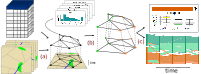
\includegraphics[width=0.95\linewidth]{overview.pdf}
    \caption{Overview of the proposed method. 
        \textbf{(a)} A network is generated from the original data,
        encoding the changing geographical information. 
        \textbf{(b)} The network is partitioned into an hierarchy. 
        \textbf{(c)} The characteristics and evolution of the clusters are then
        visually represented.
        \label{fig:overview}}
\end{figure}


\subsection{Census methodology and data representation}

Census data is disseminated in a tabulated form for aggregation areas: whole
country, state/province, metropolitan region, and so on. To allow for a more
meaningful comparison of the data, we aggregated related variables (e.g. White,
Black, Asian, Other) into what we called an \emph{aspect} (e.g. Race). The
aspects are represented using normalised histograms. This normalisation is
crucial for direct comparison. In essence, it is a generalisation of the
standard method of comparing percentages, since each aggregation area has a
different total population.

Each area of each census year is represented as a node, and edges are placed
between nodes if the corresponding regions share geographic borders in the same
year. Further, edges are placed between nodes if the corresponding regions
belong to sequential years and their geometries intersect.
To avoid spurious connections caused by small fluctuations, one of the
geometries is slightly shrunk before the intersection, using a buffer of -1e-6
degrees. While the result would not change considerably by adding more
connections between nearby regions, these extra connections would greatly
increase the computational cost. More importantly, while weights will be
associated with these edges before they are processed, they are not derived from
the geometry, but from the data. The actual intersection area is not considered
in this representation.  This approach leads to a single network representing
the whole spatio-temporal space of the data. 


\subsection{Geographic content clustering}
Having tied the regions together into a network, we can now partition it to
identify similar sets of regions. In essence, we are performing
temporal regionalisation by applying a clustering method over this
spatio-temporal network.

We start by adopting a distance function between the nodes, measuring the
difference between the data of the regions. This value is then associated with
the edges, leading to a weighted dynamic network. Every node has a collection of
histograms, each representing the distribution of certain aspect in the
population.

Let $\G=(\V,\E)$ be a network, where
$\V=\{\vertice_1,\vertice_2,\dots,\vertice_n\}$ is the set of nodes and
$\E=\{(\vertice_i,\vertice_j), i\not=j\text{ and }i,j \in [1,n]\}$ is the set of
edges. A function $\Hist$ associates each node to a set of $K$ histograms. We
define the distance $\D$ between two nodes $\vertice_i$ and $\vertice_j$ as:

\begin{equation}
    \D(\vertice_i,\vertice_j)=\sum_{k \in [1,K]}{\weight_k\, d(\Hist_k(\vertice_i),\Hist_k(\vertice_j))}
    \label{eq:dist}
\end{equation}

\noindent where $d$ is a distance metric between histograms and $\weight$ is a
sequence of non-negative weights associated with each aspect,
$\sum_{k\in[1,K]}{\weight_k}=1$. While any histogram metric can be used, we
adopted a euclidean distance between the vectors, because it led to reasonable
results with reduced computational cost. Therefore the distance between two
nodes is defined as the weighted average distance between its associated
histograms, where the weights can be adjusted by the user.

Once the distances are associated to the edges, we use watershed
cuts~\citep{Cousty2009} to create an initial clustering, which is then refined
into a hierarchy using the Sorted Maximal Matching (SMM)~\citep{markus2017}. The
initial watershed step is performed to create an initial clustering and reduce
the running time of the SMM. We introduced one new parameter to this method: a
maximum distance threshold for the merges, to avoid the early merging of
outliers. We refer the reader to the original paper~\citep{markus2017} for more
details, including a complete performance evaluation using several metrics. We
chose this algorithm because it is fast, simple, and easily customisable, but
our methodology should work with any hierarchical network clustering algorithm.
However, we caution against the use of single-linkage methods due to their
tendency to form chain-like clusters with elements that are similar pairwise,
but significantly different on the ends. That is also the reason we did not use
a Watershed hierarchy directly~\citep{najman2011equivalence}.


Each resulting cluster is contiguous in the network. This means that two
similar, but non-contiguous, sets of areas will be classified into two different
clusters, which can be counter-intuitive. To overcome this issue, we
\emph{augment} the network with two new edges per node from a nearest neighbours
graph~\citep{scikit-learn} using only the distances between the histograms.
These edges connect nodes with similar content, if they are not already
connected, providing a path for the algorithm to group similar nodes. The
regions connected by those edges will be merged on the first stages of the
clustering, since the nodes they connect are, by definition, as similar as
possible\footnote{This assertion relies on the euclidean distance and its
relationship with the space where k-nn operates.}, leaving the remaining steps
of the hierarchy to be determined only by the geographical edges. We
experimented with different numbers of augmentation edges, but the results were
not consistent, since the distribution of the edges is data dependent. Adding
two edges per node was the smallest number of edges that led to stable and
consistent results in the scenarios available in our prototype. Since the
problem of balancing the data space with the geographical space is relevant for
geographical data analysis, this idea potentially warrants further exploration,
beyond the scope of this work.


\subsection{Cluster characterisation and variable relevance}
\label{sec:relevance}
A crucial step in understanding neighbourhood change is to characterise the
evolving clusters.  The composition of each cluster is represented here by
simple statistical measures, considering each aspect separately. We compute the
minimum, maximum, median, 25\%, and 75\% quantiles for each variable of each
aspect for all clusters in the hierarchy. While interpreting these values is
more complex than interpreting just the average, they provide far more
information about the underlying distribution.


We also use these statistical measurements to discover what characterises each
cluster, that is, what makes it different from the others.  We define the
\emph{relevance} of a variable of an aspect based on the distance between the
interquartile ranges (IQR) of the clusters in the same hierarchical level. If
the IQRs overlap for all clusters, that variable is not relevant to the
characterisation of the cluster, but if the IQRs are distant, it means that this
specific range of values is something that only occurs in this cluster.
Examining IQRs therefore provides users a straightforward visual method for
determining what variables most clearly define a given cluster.

To allow for an easier visualisation of these ideas, we represent it using an
\emph{enhanced} version of the traditional boxplot, which includes the IQRs for
the other clusters, in slightly larger and faded black rectangles. We also
colour the current IQR according to its relevance, as illustrated in
Figure~\ref{fig:boxplot}. In this example, this cluster is best defined by the
proportion of the population with four or more years of college. The user can
quickly see that this is relevant because the corresponding IQR is coloured with
the highest relevance present in the legend. It is also clear that, while this
cluster includes CTs that have between 10\% to 90\% of people in this variable,
approximately, half of them have about 60\% of the population with four or more
years of college. Since all the other IQRs are well separated, this is a
defining characteristic of this cluster. Conversely, the proportion of the
population with one to three years of college is not relevant, as indicated by
black fill in the rectangle representing the IQR of this cluster, in overlapping
position with the rectangles of the other clusters.

\subsection{Clusters and trajectories}
While the partition of the data into different clusters helps the user to
understand what groups exist and where they are, we are also interested in the
evolution of these groups. To examine this process of evolution directly, we
introduce the concepts of \emph{temporal paths} and \emph{trajectories}. 

From network theory, a \emph{path} is a sequence of nodes of the network that
are connected pairwise by edges. As each node has associated temporal
information, we call \emph{temporal} any path such that the temporal information
increases along it. For instance, in Figure~\ref{fig:intuition}, the paths ACF,
ADF, ADG, and BEH are temporal paths, but not HEB, CDE, nor FDA. With harmonised
data, as illustrated by the path BEH, the time-series of each region would form
a temporal path, each node would be connected only to its older and newer
versions, and would belong to only one temporal path. Since our data is not
harmonised, more connections are allowed and each node can belong to an
arbitrary number of paths.

Semantically, this is a generalisation of the idea of geographical time-series,
because each temporal path is one possible option for the data to change over
time. Returning to Figure~\ref{fig:intuition}, the paths ACF, ADF, and ADG all
start on the same homogeneous region, but evolve differently over time. In other
words, this network encodes the information that portions of the region A
changed to form regions C and D, but we do not know specifically which parts.
Nor do we need to, since the same region can belong to several temporal paths.
Interestingly, when interpreted in this framework, geographical harmonisation is
a method to split and/or merge nodes so each belongs to a single temporal path.

Since each node in the sequence that forms the temporal paths has an associated
cluster, we can classify the paths based on the sequence of clusters. We call
each unique sequence of clusters present in this result a \emph{trajectory}.
Regions on the same trajectory had the same sequence of clusters, therefore had
similar temporal evolution.

\subsection{Overview of the prototype interface}
\label{sec:ui}
To validate and explore the results of our methodology, we built a user
interface, illustrated in Figure~\ref{fig:ui}, considering census tract (CT)
level data from the Chicago region between 1970 and 2010. This region is known
for its entrenched racial divide and the emergence of a \emph{'young urban'}
population with a higher education level~\citep{Delmelle2016,Delmelle2017}. More
details are presented in Section~\ref{sec:study}.


\begin{figure*}
    \centering 
    \includegraphics[width=0.95\linewidth]{ui.pdf}
    \caption{Initial interface of our method showing the demographic evolution of Chicago and identifying the objectives of each plot.
        \textbf{(what)}: Cluster overview illustrating the most relevant aspect for each cluster. 
        \textbf{(where)}: Maps illustrating the geographical location, both as an overall summary and for each year.
        \textbf{(how)}: Tabular and visual summary of how the regions classification changed over time.
        \textbf{(who)}: Demographic details for the currently selected data.
        \label{fig:ui}}
\end{figure*}


As illustrated by Figure~\ref{fig:ui}, our proposed interface heavily
relies on colour to express cluster-related information. We adopted
this convention because colours can be used in all our visual tools in
a coherent manner. However, there is a limit on the number of distinct
colours that can be used. We limited the number of clusters to eight
because this was the largest number of colours that we could reliably
and accessibly use, derived from the 8-class Dark2 set from
ColorBrewer~\citep{ColorBrewer}.


The configuration panel, on top left in Figure~\ref{fig:ui}, displays the
processing configuration of the visualised results: which aspects were used and
their weights (following Equation~\ref{eq:dist}). It also includes other
configuration options that can be altered without re-processing the data, such
as the number of clusters and the colour option. The gear button allows access
to the other configuration options that do require further processing, such as
changing location, aspects, and weights. 

The main functionalities of the interface allow users to examine four
inter-related questions central to understanding local area dynamics. 1)
\emph{What} do the clusters consist in?; 2) \emph{Where} are they located; 3)
\emph{How} do they change?; and 4) \emph{Who} occupy them? We discuss each in
turn.  

The cluster overview panel, marked as \emph{what} in Figure~\ref{fig:ui},
displays the most relevant aspects for each cluster, based on the distance
between the IQRs, as detailed in Section~\ref{sec:relevance}. This
feature allows the user to quickly understand what exists in this region and
which aspect makes each cluster unique, without going into excessive detail. In
Chicago's example, we expect race to be relevant in general, and indeed, it is
recognised as the most relevant aspect for three of the four most distinct
clusters, with the fourth being education level. As we increase the number of
clusters, they get more nuanced, requiring more than one aspect for their proper
characterisation, as each cluster is divided into its composing sub-clusters.
The \emph{View all} button opens a new panel where all aspects are included,
while the chevron at the side lets the user expand each cluster separately,
allowing the exploration of more details on demand.


\begin{figure}
    \centering 
    
\includegraphics[width=0.425\linewidth]{boxplot.pdf}
    \caption{Enhanced boxplot of the clusters' characteristics allows a quick
    comparison to the other clusters.\label{fig:boxplot}}
\end{figure}


With the knowledge of what clusters are present, we can explore where they are
through the maps, marked as \emph{where} in Figure~\ref{fig:ui}. While the maps
on the lower part of the interface show the location of the clusters at each
time, the larger map shows a summarised version, based on the trajectories of
each region. In simplified mode the colour corresponds to the
cluster present in that trajectory for more than half the temporal samples, and
is grey otherwise. With simplified colours disabled, the colours are the average
of the colours of the clusters in that trajectory in RGB colour
space~\footnote{\url{https://gka.github.io/chroma.js/\#chroma-average}}.

Each trajectory represents a different temporal path through the clusters.
Therefore the trajectories encode how the demographic characteristics changed
over time. These changes are summarised by the two sections identified as
\emph{how} in Figure~\ref{fig:ui}. In the left panel, there is a Sankey diagram
where each ribbon represents a different trajectory. Since the associated
regions have different population numbers, the width of each ribbon is
proportional to the smaller of the populations involved, pairwise. This
approximation works well in general, but leads to small inconsistencies in some
specific cases. For instance, in the results for Miami, which is available in
the supplementary material, the combined width of the ribbons decreases
slightly, despite an increase in the population numbers.

In our example in Figure~\ref{fig:ui}, the orange and green clusters contain
most of the population and are fairly stable over time. The pink cluster is
small and mostly stable. The purple cluster is increasing, mostly by
incorporating areas that were previously orange. Since the purple group
corresponds to the emergent 'young urban' group, this corroborates the findings
of Delmelle~\citep{Delmelle2016,Delmelle2017}, showing that our network-based
method can recover results from the traditional data processing approach.

In the next panel, illustrated in the top middle of Figure~\ref{fig:ui}, is a
transition matrix between the clusters. It indicates a rounded percentage of
regions whose area changed between each pair of clusters. In this example, we
can see that all clusters are fairly stable, with more than ninety percent of
identity transitions. This kind of table can be found in the related
literature~\citep{Delmelle2016}, so it is familiar to the advanced users. It not
only informs the proportional changes, but allows the selection of specific
changes for further analysis.


The bottom part of the interface contains the details for the selected
trajectories, or for the whole city if nothing is selected, marked as \emph{who}
in Figure~\ref{fig:ui}. The stacked bar plots summarise the overall demographic
composition of these regions. In this example, the maps show the transition from
orange to green and purple in several regions over time. Each aspect is
represented by a stacked bar plot, where the width of each rectangle corresponds
to the percentage of population in that variable over the considered period. In
this case, a little less than half of the population are married, and the
percentage that are Widowers or Divorced is roughly similar. About half of the
population work in Administrative jobs, a third never completed high-school,
approximately forty percent have gross family income below 50,000USD per year.
About sixty percent identify as white. Placing the mouse over one of the bars
will open a small panel with the temporal evolution of the population percentage
of that specific variable, and clicking on the chevron on the right side expands
the corresponding aspect, showing census tract level statistics, with details of
the temporal evolution of each variable and also the corresponding IQRs for the
whole city. Those values differ from the total population percentage. While the
overall population of this region is about sixty percent White, the average
percentage of White population over the CTs is a little over forty percent.

More importantly, this interface is fully interactive, allowing for a
progressive exploration of the data. Clicking on a cluster in the cluster
overview panel and the other panels will filter the results to consider only
that cluster, highlighting the geographic regions and involved changes, and
updating population count and demographic composition. If the user selects a
region from the larger map, all identical trajectories are considered, and the
whole interface changes to allow for further study of that specific region.
Clicking on a region in small maps will bring up a new panel with the original
census data of this specific region. Further, these selectors can be combined in
different ways, enabling complex queries with instantaneous results.


\section{Illustrative scenarios}
\label{sec:study}

In this section we present two illustrative scenarios, using census data from
the United States~\citep{nhgis} and
Canada\footnote{\url{http://datacentre.chass.utoronto.ca/census/}}, tabulated by
CTs,  from 1970 to 2010. 

The prototype interface allows access to 41 regions, 29
in the US and 12 in Canada. New York City was split into its boroughs to avoid
memory crashes on the client browser due to the high number of CTs.  We used
five aspects for the USA: Education level, Family income, Marital status,
Occupation, and Race; and seven for Canada: Age, Education level, Home language,
Household Income, Marital status, Occupation, Place of birth, and Religion. 

While our method does not require geographic harmonisation, it requires matching
the variables over time. The supplementary material contains the details of
which census columns were used for each aspect. Income is slightly inaccurate,
even though we did correct for the official inflation. We grouped the original
ranges into three larger ranges, but they do not match precisely.

\unsure{CHECK}\revision{1.12.(1-5)}{These results are meant to demonstrate the
utility of the interface for understanding the evolutionary dynamics of urban
neighbourhoods. They also show the face validity of the results generated by our
novel network-based approach. However, the US data for 2010 is  not from the
decennial census, but from the ACS 2006-2010, compromising the temporal
stability of the data. Further, the regions selected do not correspond to any
pre-defined regions (metros, cities, census areas), but to somewhat arbitrary
regions defined around a location of interest, making direct comparisons harder.
Since  variable matching is a  manual process, we selected a minimal set of
aspects for each country, which are not necessarily similar to each other, or
similar to studies in the current literature. These factors would seriously
hinder any study using the existing methods, but our results were well-aligned
with several other studies, illustrating the robustness of our approach to
imperfect conditions. }

\subsection{Chicago}
Our first scenario examines Chicago, using an arbitrary region larger than the
administrative borders. Its demographic composition is well explored in the
literature, with reports of racial divide and
gentrification~\citep{Delmelle2016,Delmelle2017,Hwang2014}, so we expect our
results to contain stable regions where the Race aspect is relevant, and some
degree of population change, with increasing income and education levels. 


The initial state of the prototype is illustrated in Figure~\ref{fig:ui}. The
first step is to identify the compositions of each cluster from the boxplots, so
orange is associated with majority of White population, green with majority
Black, and purple with higher proportion of four years of college or more (high
education level). The expanded version of the boxplots for the purple cluster
shows a higher income level and majority of occupations in administrative jobs,
therefore the purple cluster identifies gentrified regions.


The trajectories plot illustrates the process of gentrification, also
illustrated in Figure~\ref{fig:chiWorkflow}, progressively absorbing regions
from the orange cluster (White). This corroborates results from the literature
reporting that Black neighbourhoods are less likely to
gentrify~\citep{Hwang2014}. The transition matrix provides more details, showing
that around one percent of all regions that became purple at any time
transitioned from the green cluster (Black population), while nine percent were
previouly associated with the orange cluster (White). Next, we select the region
that is gentrified in 2010, by clicking on the corresponding rectangle in the
trajectories plot, updating the information on the maps and the details portion
of the interface.

The corresponding regions are highlighted in the maps, where the spatial pattern
is clear, corresponding exactly to previous findings in the literature based
upon harmonisation~\citep{Hwang2014}. Further, we can also identify the regions
that gentrified earlier on the small maps that depict the involved regions over
time. Since the most relevant aspect is Education, specifically "Four or more
years of college", we can expand the details of this aspect, as illustrated in
the rightmost portion of Figure~\ref{fig:chiWorkflow}, which is increasing for
the whole city (grey band), but faster and to a higher level in this region
(black band).



\begin{figure*}
    \centering
 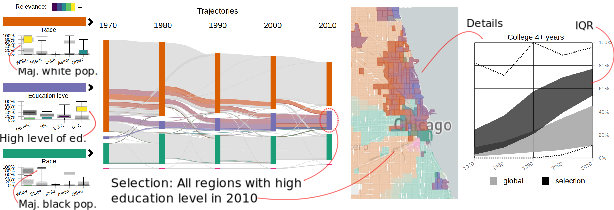
\includegraphics[width=0.9\linewidth]{newTeaser.pdf}
 \caption{Workflow to discover gentrification in Chicago: the purple cluster
 corresponds to high education / income. Its population is increasing over time,
 absorbing from the majority White cluster (orange). By selecting the purple
 cluster in 2010, the region is highlighted in the maps. The proportion of
 people with 4+ years of college is increasing in the whole city (grey IQRs),
 but significantly more in this region (black).\label{fig:chiWorkflow}}
\end{figure*}



\subsection{Toronto}

We consider a region that corresponds approximately to the administrative border
of the current city of Toronto, using all seven available aspects with equal
weights. While Chicago was fairly stable, Toronto is known to be a more dynamic
and diverse city, with significant and increasing immigrant
population~\citep{hulchanski2007three,Fong2011}, especially
Asian~\citep{Fong2003}. Toronto is also known for a stable and well defined
Jewish community~\citep{Harold2018, Fong2011}. Therefore, we expect \revision{1.14}{a}
combination of stable and dynamic regions on the results, with Place of Birth,
Home Language, and Religion identified as relevant aspects. The results are
summarised in Figure~\ref{fig:to}, considering eight clusters.

\begin{figure}
    \centering 
    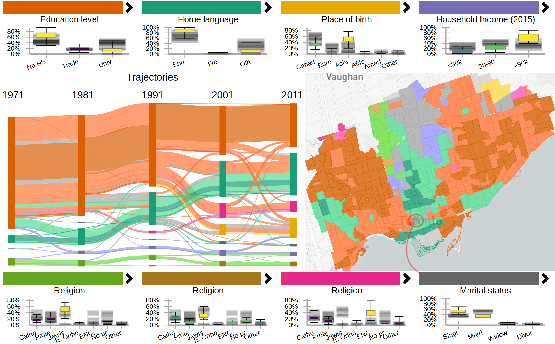
\includegraphics[width=0.85\linewidth]{to.pdf}
    \caption{Clustering results for Toronto, with eight clusters, including
    clusters representing Jewish population, high and low income, low education,
    and Asian immigration.\label{fig:to}}
\end{figure}

The population with low percentage of University degrees is represented in
orange, mostly anglophone population in green, Asian immigrants in yellow, high
percentage of income in the highest bracket in purple, high percentage of Jewish
people in light green and brown, high percentage of Eastern Non-Christian
religion in pink, and high concentration of single people in dark grey. From the
trajectories plot, we can see that Toronto is more dynamic than Chicago, with
one cluster constantly shrinking. In the 1970s, the city was divided into four
clusters: low number of university degrees, Jewish population, majority
anglophones, and high income. Interestingly, the more recent clusters that
absorbed regions from the orange cluster have similar education profiles and are
differentiated by other aspects. In this sense, the city is growing diverse,
changing from a common low education profile to a higher level of education with
more diversity in religion (pink) and immigration (yellow).


Indeed, the growing Asian population is visible starting in the 1980s and
building thereafter, leading to the yellow and pink clusters. While both include
a high percentage of people born in Asia, the pink is more defined by religion,
with low percentage of university degrees, and contains the lowest percentage of
people in the highest income bracket for these clusters; the yellow is less
defined by religion, and has higher education and income, geographically
corresponding to the Markham region, know for its Chinese population. A similar
division also happens for the two Jewish clusters, where the light green cluster
has lower education and income levels than the brown cluster. The purple cluster
of high income is somewhat stable. Until 2011 the cluster included the Bridle
Path neighbourhood, known for its wealthy population. In 2011 it was classified
into the yellow cluster of Asian immigration, since about 40\% of the population
for this CT were then born in Asia. The income distribution did not change, with
85\% of the population with an income of 90k CAD or more.


The most significant indicator of Toronto's dynamism is the presence of grey
regions on the map. These represent regions associated to three or more clusters
over this five census period. Using the 'Add' mode for the trajectory selection,
we select their trajectories, and a subset of the details is illustrated in
Figure~\ref{fig:toVol}. These regions account for about 5\% of Toronto's
population. The whole region was classified into the orange cluster in 1971 (low
level of university degrees). By 1991, most of the region was classified into
the green cluster, representing anglophone population, mostly Canadian born,
with a higher level of education. As the corresponding plot indicates, this
trend in increasing education is city-wide, but this region has people with
better education than most.

\begin{figure}
    \centering 
    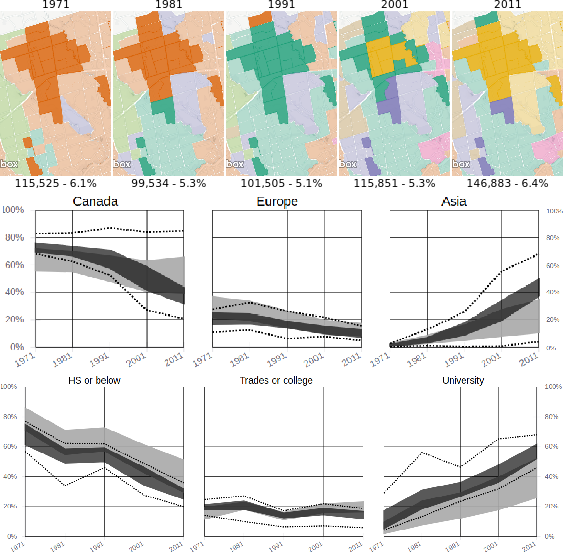
\includegraphics[width=0.75\linewidth]{toVol.pdf}
    \caption{Details for some regions of Toronto that were classified into 3 or
         more clusters over time.\label{fig:toVol}}
\end{figure}

In 2001, the purple cluster of high income annexes neighbouring parts of the
volatile region, and the Asian born population increases sharply, as illustrated
by the appearance of the yellow cluster.  This cluster indicates well educated,
higher income, and about 30\%-50\% Asian born population. By 2011, the yellow
cluster increased considerably, annexing parts of the high income purple
cluster, including the neighbouring Bridle Path area.

The geographical borders of the clusters obtained using our method are similar
to the regions presented by previous studies considering
Toronto~\citep{hulchanski2007three}. However, our interface provides a deeper
insight into their demographic composition, since we consider more data than
solely Average Income, which appears to be a good proxy variable nonetheless.
This scenario showcases the ability of our method and interface to capture and
understand the sources of urban volatility.

\section{Expert feedback}
\label{sec:expert}
As our method and tool are novel to the field, and somewhat exotic,  we
subjected them to the critical scrutiny of experts. We contacted academic and
industry experts in sociology and urban sciences to solicit their evaluation of
our methodology. They had access to the prototype tool, a descriptive
documentation of the features (included in the supplementary material), and a
sequence of documentation videos illustrating how to perform specific tasks. The
documentation explains which datasets are used and how the data is represented
and processed, noting explicitly that there is no geographic harmonisation. We
focused our inquires on the results obtained, asking if they found anything
interesting in the data. The message sent and their full response is included in
the supplementary material. Each of the five experts is identified by a letter,
from A to E. 



The overall overall response of the experts was positive,  mentioning that the
prototype allows them to analyse census data without the additional work of
obtaining and cleaning the data (A, B, E), and it allows the inclusion of
geographic visual analysis tools in their research process (D). It enables the
users to tell different stories about neighbourhoods/cities and their changes
(A), visualise the relationship between key urban variables over time (D),
offering a quick way to identify particular neighbourhoods that one may be
interested in studying more in depth around a particular issue or efficiently
understanding the context of an area (E).  Indeed, the experts identified
gentrification processes in Manhattan (B) and Dallas (E), reinforced a
hypothesis for occupational clustering (D), and highlighted how the method can
be used to compare neighbourhoods and cities (A). In summary, their view was that
the proposed methodology can be a viable alternative for the visual analytics of
evolving demographic data.



The interface was "easy to navigate" (B), but it was also considered
"overwhelming" (A), "intimidating" (E), and "tricky to interpret" (C), possible
side-effects of our effort to increase  representational accuracy, where we
avoided using simplified representation or labels. Identifying clusters by their
most relevant variables was welcome, but the overlap of information from
different clusters in the boxplot was "a bit confusing" (C) when colour was not
present. Further, most clusters can be sufficiently characterised using only the
most relevant aspect, but this is not generally true. 


While the map of trajectories was mentioned as a "good summary map", how it
related to the clustering method was unclear (C). The methods include different
options on how the colours are used, but both are works in progress since reliably
representing several distinct entities using colours is humanly unfeasible.
Indeed, the number of distinguishable colours was a significant constraint, we
found indications that more clusters should be used in some cases, even if eight
clusters is more than what is traditionally considered in these analyses.
Conversely, increasing the number of clusters would also complicate the
interpretation of the results.


The experts also mentioned the poor responsiveness of the method when changes in
the clustering parameters required server-side processing (B,D). Indeed, the
current implementation can take a few minutes to cluster regions with high
number of CTs, like Los Angeles or Brooklyn. Server-side processing reduced the
amount of data transferred to client, but it might increase the response time
under load. We implemented a caching policy, but fully pre-processing the
results is not practical due to size of the parameter space.

Most of the experts demonstrated interest in using our method in their research
(A, B, D, E), aiming to use the census data as a backdrop for other datasets,
providing demographic context. They also mentioned the need to export subsets of
data, plots, and maps to be used in reports and publications (C, D, E). More
importantly, while these experts were aware that our method does not perform
geographic harmonisation, none of them mention it. We did not specifically ask
if this difference led to unexpected results, but rather if they found
interesting insights. 

\section{Discussion and limitations}
\label{sec:discussion}

Our objective was to leverage a network based data representation and
visualisation methods for the exploration of geographically inconsistent
region-based data. While we successfully replicated and corroborated results
from the literature, this method still has significant limitations. 


Removing the need for geographical harmonisation greatly reduces the amount of
work necessary to explore demographic data, but the method still requires
consistent variables across the years. Matching the variables can be trivial for
some aspects (Age), but challenging for others (Income). The divulged income
ranges vary over time and the actual values change due to inflation. Some
variables were not considered in earlier censuses, such as Race in Canada, or
Hispanic population in the USA, hampering its use when they are available. Since
this is only a prototype, we matched few aspects, but a proper demographic
analysis would benefit from all available information. 

The limitation on the number of displayed clusters because of the limited number
of distinguishable colours was significant. While increasing the number of
clusters would further complicate an already complex analysis, it might be
warranted for some regions. Colour is a fundamental and intuitive tool for
information representation that can be coherently used across different plots,
so we opted to use it, even if in a limited way. With eight colours, there was
overlap between some clusters, the relevance gradient, and the colour
combination. 


The cognitive load on the user is significant, as we compromised simplicity for
accuracy. While other works labelled the clusters, as 'young urban',
'struggling', and so on~\citep{Delmelle2016,Delmelle2017}, we show the
statistical characteristics of the clusters, which are harder to interpret, as
the data may have subtle nuances that labels would otherwise hide. This also led
to a crowded interface, mitigated somewhat the use of pop-up panels and
collapsible sections. For some cities, especially if they are small and stable,
the panels can appear redundant, but each provide a different way to interact
with the information that can ease the exploration process for larger and
dynamic cities.

\section{Conclusions}
Our objective was to allow for the exploration of census data without
geographical normalization, an approach that is usually not considered:
\emph{"(...) tract-by-tract comparison is not possible unless data from 2000 is
interpolated to 2010 boundaries (...)"}~\cite{Dmowska2017}. Our method was able
to corroborate previous findings from the specialized literature, with an
increased level of detail due to our data representation and visualization
choices. The feedback from experts was remarkably positive, most of them were
able to extract insight from the prototype and demonstrated interest in using it
on their research efforts.

While we focused on census data in this work, the proposed method can be used
with most similarly area-based datasets. Further, while there is interest in the
use of census data, it is mostly in combination with other, larger and more
dynamic, datasets. We postulate that, while census data is interesting, the
amount of effort required to obtain and prepare it often discourages its use as
complementary information, reinforcing our hypothesis that there is need for
methods that are able to deal with geographically inconsistent data. 



%% if specified like this the section will be ommitted in review mode
\acknowledgments{This research was supported by a University of Toronto
Connaught Global Challenge grant and is part of the Urban Genome Project.}
\bibliographystyle{abbrv-doi-hyperref-narrow}

\bibliography{rev}
\end{document}
